\documentclass{standalone}
\usepackage{tikz}
\usetikzlibrary{calc}
\usetikzlibrary{automata, positioning, arrows}
\tikzstyle{inarrow}=[->, >=stealth, shorten >=-.03cm,line width=0.5]
\begin{document}
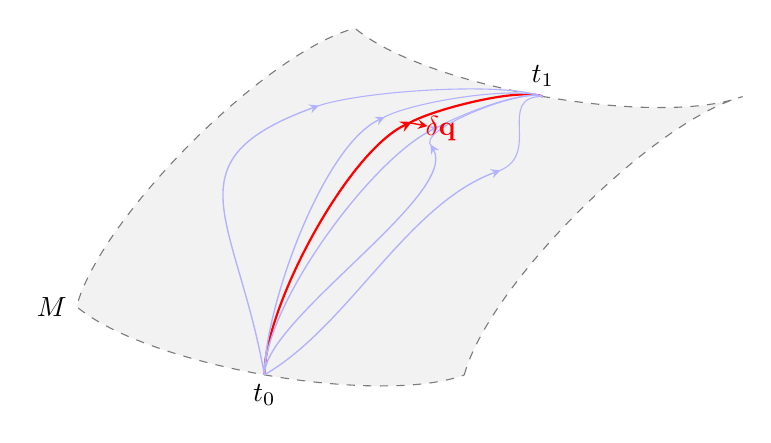
\begin{tikzpicture}[x={({cos(-10)*1cm},{sin(-10)*1cm})},y={({cos(45)*1cm},{sin(45)*1cm})},z={(0,1cm)}]
  \draw[dashed, fill=gray!20, opacity=0.5, looseness=.6] 
    (2.5,-2.5,-1)
    to[bend left] coordinate (mk) (2.5,2.5,-1)
    to[bend left] coordinate (mp) (-2.5,2.5,-1) 
    to[bend right] coordinate (mq) (-2.5,-2.5,-1) coordinate (labelM)
    to[bend right] coordinate (mm) (2.5,-2.5,-1)
    -- cycle;
  \node[left] at (labelM) {$M$};
  % \draw[fill=gray!20, opacity=0.2] 
  %   (2.5,-2.5,0)
  %   -- (2.5,2.5,0) 
  %   -- (-2.5,2.5,0)
  %   -- (-2.5,-2.5,0) coordinate (labelTM) 
  %   -- cycle;
  % \node[above right, label=left:$T_\mathbf{q}M$] at (labelTM) {};
  \draw[inarrow, thick, red,looseness=.6] (mm) to[in=205, out=90] (0,0,0);
    \draw[thick, red, looseness=.5] (0,0,0) to[out=30, in=160] (mp);

  \draw[inarrow, blue!30, looseness=.6] (mm) to[in=205, out=90] (-0.35,0,0);
    \draw[blue!30, looseness=.5] (-0.35,0,0) to[out=30, in=160] (mp);

  \draw[inarrow, blue!30, looseness=.6] (mm) to[in=205, out=90] (0.35,0,0);
    \draw[blue!30, looseness=.5] (0.35,0,0) to[out=30, in=160] (mp);

  \draw[inarrow, blue!30,looseness=.5] (mm) to[in=300, out=90] (0.5,-0.3,0);
    \draw[blue!30,looseness=.5] (0.5,-0.3,0) to[out=140, in=160] (mp);
  
  \draw[inarrow, blue!30,looseness=0.8] (mm) to[in=200, out=30] (1.5,-0.5,0);
    \draw[blue!30,looseness=1.4] (1.5,-0.5,0) to[out=20, in=180] (mp);

  \draw[inarrow, blue!30,looseness=1.5] (mm) to[in=200, out=100] (-1.2,0,0);
    \draw[blue!30,looseness=.5] (-1.2,0,0) to[out=20, in=160] (mp);
  %\node (q) at (0,0,0) {\textbullet};
    \node[below] at (mm) {$t_0$};
    \node[above] at (mp) {$t_1$};
  \draw[inarrow, red] (0,0,0) -- (0.2,0,0);
    \node[red] at (0.4,0,0) {$\delta\mathbf{q}$};
  
\end{tikzpicture}
\end{document}